\section{Parte II}

En esta segunda parte describiremos el resultado del sprint, incluyendo las secciones seguimiento, product increment, retrospectiva y de diseño orientado a objetos.
 
La misma es una revisi\'on de la entrega anterior del documento de acuerdo a las correcciones y anotaciones realizadas.


\subsection{Seguimiento}
\subsubsection{Beneficio del framework Scrum}

La utilizaci\'on de Scrum para el manejo del proyecto nos brindó muchos beneficios en la primer etapa de an\'alis siendo una herramienta de mucha ayuda al descomponer los requerimientos en user stories y luego en tareas. 

Sin embargo, al no poder realizar actualización de horas retroactivas, algo bastante común de realizar en otras herramientas de seguimiento, el burnout chart no es fiel reflejo de nuestro avance. Esto nos sucedió ya que al mantener un constante intercambio de mails nos di\'o la visibilidad del avance suficiente que nos hizo olvidar del uso de la herramienta para esto.

Adicionalmente respecto del seguimiento del proyecto, utilizando la asignaci\'on de tareas por intermedio de RallyDev no nos result\'o beneficiosa. Principalmente porque las asignaciones iniciales las fuimos cambiando durante el sprint dependiendo de la necesidad de avanzar sobre ciertos punto y de los tiempos disponibles de cada uno, con lo cual andar reflejando constantemente los cambios hubiera resultado en un mayor trabajo.

\subsubsection{Burndown chart}
\begin{figure}[ht]
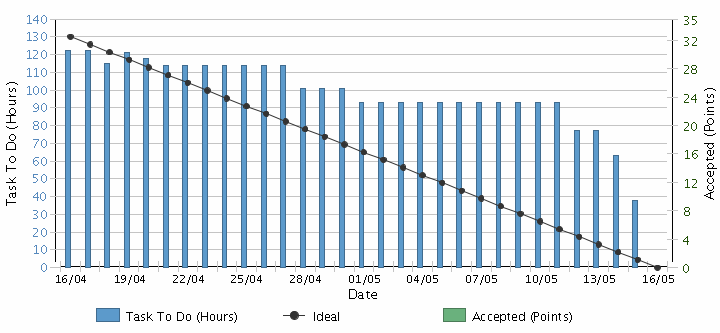
\includegraphics[width=\textwidth]{./imgs/burndown.png}
\end{figure}
